\documentclass{standalone}
\usepackage{tikz}
\usetikzlibrary{shapes}
\begin{document}
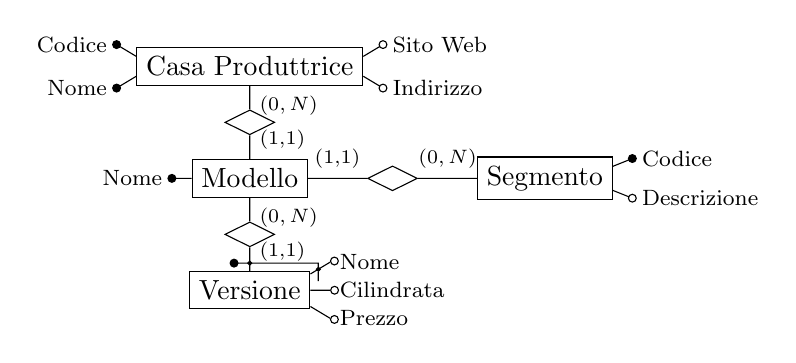
\begin{tikzpicture}
    \draw

    
    (0,0)node[draw, rectangle](casa){Casa Produttrice}

    (casa.175)--++(-0.25, 0.15)node[draw, circle, inner sep=1pt, fill=black]{}node[left]{\footnotesize Codice}
    (casa.185)--++(-0.25,-0.15)node[draw, circle, inner sep=1pt, fill=black]{}node[left]{\footnotesize Nome}
    (casa.355)--++( 0.25,-0.15)node[draw, circle, inner sep=1pt, fill=white]{}node[right]{\footnotesize Indirizzo}
    (casa.5) --++( 0.25, 0.15)node[draw, circle, inner sep=1pt, fill=white]{}node[right]{\footnotesize Sito Web}


    (casa.270)node[below right]{\scriptsize $(0,N)$}--++(0,-0.3)node[draw, diamond, shape aspect=2, inner sep=3pt, anchor=90](r1){}
    (r1.270)--++(0,-0.3)node[above right]{\scriptsize (1,1)}node[draw, rectangle, anchor=90](modello){Modello}
    (modello.180)--++(-0.25,0)node[draw, circle, inner sep=1pt, fill=black]{}node[left]{\footnotesize Nome}

    (modello.0)--++(0.75,0)node[midway, above]{\scriptsize (1,1)}node[draw, diamond, shape aspect=2, inner sep=3pt, anchor=180](r3){}
    (r3.0)--++(0.75,0)node[midway, above]{\scriptsize $(0,N)$}node[draw, rectangle, anchor=180](segmento){Segmento}
    (segmento.10)--++(0.25,0.1)node[draw, circle, inner sep=1pt, fill=black]{}node[right]{\footnotesize Codice}
    (segmento.350)--++(0.25,-0.1)node[draw, circle, inner sep=1pt, fill=white]{}node[right]{\footnotesize Descrizione}


    (modello.270)node[below right]{\scriptsize $(0,N)$}--++(0,-0.3)node[draw, diamond, shape aspect=2, inner sep=3pt, anchor=90](r2){}
    (r2.270)--++(0,-0.2)node[draw, circle, inner sep=0.5pt,fill=black](a){}--++(0,-0.1)node[above right]{\scriptsize (1,1)}node[draw, rectangle, anchor=90](versione){Versione}
    (versione.15)--++(0.1,0.06)node[draw, circle, inner sep=0.5pt,fill=black](b){}--++(0.15,0.09)node[draw, circle, inner sep=1pt, anchor=195]{}node[right]{\footnotesize Nome}
    (versione.0)--++(0.25,0)node[draw, circle, inner sep=1pt,anchor=180]{}node[right]{\footnotesize Cilindrata}
    (versione.345)--++(0.25,-0.15)node[draw, circle, inner sep=1pt,anchor=165]{}node[right]{\footnotesize Prezzo}
    
    (a)++(-0.2,0)node[draw, circle, inner sep=1pt, fill=black](){}-|(b)--++(0,-0.15)


    ;    
\end{tikzpicture}
\end{document}